\documentclass[11pt]{article}

    \usepackage[breakable]{tcolorbox}
    \usepackage{parskip} % Stop auto-indenting (to mimic markdown behaviour)
    
    \usepackage{iftex}
    \ifPDFTeX
    	\usepackage[T1]{fontenc}
    	\usepackage{mathpazo}
    \else
    	\usepackage{fontspec}
    \fi

    % Basic figure setup, for now with no caption control since it's done
    % automatically by Pandoc (which extracts ![](path) syntax from Markdown).
    \usepackage{graphicx}
    % Maintain compatibility with old templates. Remove in nbconvert 6.0
    \let\Oldincludegraphics\includegraphics
    % Ensure that by default, figures have no caption (until we provide a
    % proper Figure object with a Caption API and a way to capture that
    % in the conversion process - todo).
    \usepackage{caption}
    \DeclareCaptionFormat{nocaption}{}
    \captionsetup{format=nocaption,aboveskip=0pt,belowskip=0pt}

    \usepackage[Export]{adjustbox} % Used to constrain images to a maximum size
    \adjustboxset{max size={0.9\linewidth}{0.9\paperheight}}
    \usepackage{float}
    \floatplacement{figure}{H} % forces figures to be placed at the correct location
    \usepackage{xcolor} % Allow colors to be defined
    \usepackage{enumerate} % Needed for markdown enumerations to work
    \usepackage{geometry} % Used to adjust the document margins
    \usepackage{amsmath} % Equations
    \usepackage{amssymb} % Equations
    \usepackage{textcomp} % defines textquotesingle
    % Hack from http://tex.stackexchange.com/a/47451/13684:
    \AtBeginDocument{%
        \def\PYZsq{\textquotesingle}% Upright quotes in Pygmentized code
    }
    \usepackage{upquote} % Upright quotes for verbatim code
    \usepackage{eurosym} % defines \euro
    \usepackage[mathletters]{ucs} % Extended unicode (utf-8) support
    \usepackage{fancyvrb} % verbatim replacement that allows latex
    \usepackage{grffile} % extends the file name processing of package graphics 
                         % to support a larger range
    \makeatletter % fix for grffile with XeLaTeX
    \def\Gread@@xetex#1{%
      \IfFileExists{"\Gin@base".bb}%
      {\Gread@eps{\Gin@base.bb}}%
      {\Gread@@xetex@aux#1}%
    }
    \makeatother

    % The hyperref package gives us a pdf with properly built
    % internal navigation ('pdf bookmarks' for the table of contents,
    % internal cross-reference links, web links for URLs, etc.)
    \usepackage{hyperref}
    % The default LaTeX title has an obnoxious amount of whitespace. By default,
    % titling removes some of it. It also provides customization options.
    \usepackage{titling}
    \usepackage{longtable} % longtable support required by pandoc >1.10
    \usepackage{booktabs}  % table support for pandoc > 1.12.2
    \usepackage[inline]{enumitem} % IRkernel/repr support (it uses the enumerate* environment)
    \usepackage[normalem]{ulem} % ulem is needed to support strikethroughs (\sout)
                                % normalem makes italics be italics, not underlines
    \usepackage{mathrsfs}
    

    
    % Colors for the hyperref package
    \definecolor{urlcolor}{rgb}{0,.145,.698}
    \definecolor{linkcolor}{rgb}{.71,0.21,0.01}
    \definecolor{citecolor}{rgb}{.12,.54,.11}

    % ANSI colors
    \definecolor{ansi-black}{HTML}{3E424D}
    \definecolor{ansi-black-intense}{HTML}{282C36}
    \definecolor{ansi-red}{HTML}{E75C58}
    \definecolor{ansi-red-intense}{HTML}{B22B31}
    \definecolor{ansi-green}{HTML}{00A250}
    \definecolor{ansi-green-intense}{HTML}{007427}
    \definecolor{ansi-yellow}{HTML}{DDB62B}
    \definecolor{ansi-yellow-intense}{HTML}{B27D12}
    \definecolor{ansi-blue}{HTML}{208FFB}
    \definecolor{ansi-blue-intense}{HTML}{0065CA}
    \definecolor{ansi-magenta}{HTML}{D160C4}
    \definecolor{ansi-magenta-intense}{HTML}{A03196}
    \definecolor{ansi-cyan}{HTML}{60C6C8}
    \definecolor{ansi-cyan-intense}{HTML}{258F8F}
    \definecolor{ansi-white}{HTML}{C5C1B4}
    \definecolor{ansi-white-intense}{HTML}{A1A6B2}
    \definecolor{ansi-default-inverse-fg}{HTML}{FFFFFF}
    \definecolor{ansi-default-inverse-bg}{HTML}{000000}

    % commands and environments needed by pandoc snippets
    % extracted from the output of `pandoc -s`
    \providecommand{\tightlist}{%
      \setlength{\itemsep}{0pt}\setlength{\parskip}{0pt}}
    \DefineVerbatimEnvironment{Highlighting}{Verbatim}{commandchars=\\\{\}}
    % Add ',fontsize=\small' for more characters per line
    \newenvironment{Shaded}{}{}
    \newcommand{\KeywordTok}[1]{\textcolor[rgb]{0.00,0.44,0.13}{\textbf{{#1}}}}
    \newcommand{\DataTypeTok}[1]{\textcolor[rgb]{0.56,0.13,0.00}{{#1}}}
    \newcommand{\DecValTok}[1]{\textcolor[rgb]{0.25,0.63,0.44}{{#1}}}
    \newcommand{\BaseNTok}[1]{\textcolor[rgb]{0.25,0.63,0.44}{{#1}}}
    \newcommand{\FloatTok}[1]{\textcolor[rgb]{0.25,0.63,0.44}{{#1}}}
    \newcommand{\CharTok}[1]{\textcolor[rgb]{0.25,0.44,0.63}{{#1}}}
    \newcommand{\StringTok}[1]{\textcolor[rgb]{0.25,0.44,0.63}{{#1}}}
    \newcommand{\CommentTok}[1]{\textcolor[rgb]{0.38,0.63,0.69}{\textit{{#1}}}}
    \newcommand{\OtherTok}[1]{\textcolor[rgb]{0.00,0.44,0.13}{{#1}}}
    \newcommand{\AlertTok}[1]{\textcolor[rgb]{1.00,0.00,0.00}{\textbf{{#1}}}}
    \newcommand{\FunctionTok}[1]{\textcolor[rgb]{0.02,0.16,0.49}{{#1}}}
    \newcommand{\RegionMarkerTok}[1]{{#1}}
    \newcommand{\ErrorTok}[1]{\textcolor[rgb]{1.00,0.00,0.00}{\textbf{{#1}}}}
    \newcommand{\NormalTok}[1]{{#1}}
    
    % Additional commands for more recent versions of Pandoc
    \newcommand{\ConstantTok}[1]{\textcolor[rgb]{0.53,0.00,0.00}{{#1}}}
    \newcommand{\SpecialCharTok}[1]{\textcolor[rgb]{0.25,0.44,0.63}{{#1}}}
    \newcommand{\VerbatimStringTok}[1]{\textcolor[rgb]{0.25,0.44,0.63}{{#1}}}
    \newcommand{\SpecialStringTok}[1]{\textcolor[rgb]{0.73,0.40,0.53}{{#1}}}
    \newcommand{\ImportTok}[1]{{#1}}
    \newcommand{\DocumentationTok}[1]{\textcolor[rgb]{0.73,0.13,0.13}{\textit{{#1}}}}
    \newcommand{\AnnotationTok}[1]{\textcolor[rgb]{0.38,0.63,0.69}{\textbf{\textit{{#1}}}}}
    \newcommand{\CommentVarTok}[1]{\textcolor[rgb]{0.38,0.63,0.69}{\textbf{\textit{{#1}}}}}
    \newcommand{\VariableTok}[1]{\textcolor[rgb]{0.10,0.09,0.49}{{#1}}}
    \newcommand{\ControlFlowTok}[1]{\textcolor[rgb]{0.00,0.44,0.13}{\textbf{{#1}}}}
    \newcommand{\OperatorTok}[1]{\textcolor[rgb]{0.40,0.40,0.40}{{#1}}}
    \newcommand{\BuiltInTok}[1]{{#1}}
    \newcommand{\ExtensionTok}[1]{{#1}}
    \newcommand{\PreprocessorTok}[1]{\textcolor[rgb]{0.74,0.48,0.00}{{#1}}}
    \newcommand{\AttributeTok}[1]{\textcolor[rgb]{0.49,0.56,0.16}{{#1}}}
    \newcommand{\InformationTok}[1]{\textcolor[rgb]{0.38,0.63,0.69}{\textbf{\textit{{#1}}}}}
    \newcommand{\WarningTok}[1]{\textcolor[rgb]{0.38,0.63,0.69}{\textbf{\textit{{#1}}}}}
    
    
    % Define a nice break command that doesn't care if a line doesn't already
    % exist.
    \def\br{\hspace*{\fill} \\* }
    % Math Jax compatibility definitions
    \def\gt{>}
    \def\lt{<}
    \let\Oldtex\TeX
    \let\Oldlatex\LaTeX
    \renewcommand{\TeX}{\textrm{\Oldtex}}
    \renewcommand{\LaTeX}{\textrm{\Oldlatex}}
    % Document parameters
    % Document title
    \title{Chapter 13 - Binary Heaps}
    
    
    
    
    
% Pygments definitions
\makeatletter
\def\PY@reset{\let\PY@it=\relax \let\PY@bf=\relax%
    \let\PY@ul=\relax \let\PY@tc=\relax%
    \let\PY@bc=\relax \let\PY@ff=\relax}
\def\PY@tok#1{\csname PY@tok@#1\endcsname}
\def\PY@toks#1+{\ifx\relax#1\empty\else%
    \PY@tok{#1}\expandafter\PY@toks\fi}
\def\PY@do#1{\PY@bc{\PY@tc{\PY@ul{%
    \PY@it{\PY@bf{\PY@ff{#1}}}}}}}
\def\PY#1#2{\PY@reset\PY@toks#1+\relax+\PY@do{#2}}

\expandafter\def\csname PY@tok@w\endcsname{\def\PY@tc##1{\textcolor[rgb]{0.73,0.73,0.73}{##1}}}
\expandafter\def\csname PY@tok@c\endcsname{\let\PY@it=\textit\def\PY@tc##1{\textcolor[rgb]{0.25,0.50,0.50}{##1}}}
\expandafter\def\csname PY@tok@cp\endcsname{\def\PY@tc##1{\textcolor[rgb]{0.74,0.48,0.00}{##1}}}
\expandafter\def\csname PY@tok@k\endcsname{\let\PY@bf=\textbf\def\PY@tc##1{\textcolor[rgb]{0.00,0.50,0.00}{##1}}}
\expandafter\def\csname PY@tok@kp\endcsname{\def\PY@tc##1{\textcolor[rgb]{0.00,0.50,0.00}{##1}}}
\expandafter\def\csname PY@tok@kt\endcsname{\def\PY@tc##1{\textcolor[rgb]{0.69,0.00,0.25}{##1}}}
\expandafter\def\csname PY@tok@o\endcsname{\def\PY@tc##1{\textcolor[rgb]{0.40,0.40,0.40}{##1}}}
\expandafter\def\csname PY@tok@ow\endcsname{\let\PY@bf=\textbf\def\PY@tc##1{\textcolor[rgb]{0.67,0.13,1.00}{##1}}}
\expandafter\def\csname PY@tok@nb\endcsname{\def\PY@tc##1{\textcolor[rgb]{0.00,0.50,0.00}{##1}}}
\expandafter\def\csname PY@tok@nf\endcsname{\def\PY@tc##1{\textcolor[rgb]{0.00,0.00,1.00}{##1}}}
\expandafter\def\csname PY@tok@nc\endcsname{\let\PY@bf=\textbf\def\PY@tc##1{\textcolor[rgb]{0.00,0.00,1.00}{##1}}}
\expandafter\def\csname PY@tok@nn\endcsname{\let\PY@bf=\textbf\def\PY@tc##1{\textcolor[rgb]{0.00,0.00,1.00}{##1}}}
\expandafter\def\csname PY@tok@ne\endcsname{\let\PY@bf=\textbf\def\PY@tc##1{\textcolor[rgb]{0.82,0.25,0.23}{##1}}}
\expandafter\def\csname PY@tok@nv\endcsname{\def\PY@tc##1{\textcolor[rgb]{0.10,0.09,0.49}{##1}}}
\expandafter\def\csname PY@tok@no\endcsname{\def\PY@tc##1{\textcolor[rgb]{0.53,0.00,0.00}{##1}}}
\expandafter\def\csname PY@tok@nl\endcsname{\def\PY@tc##1{\textcolor[rgb]{0.63,0.63,0.00}{##1}}}
\expandafter\def\csname PY@tok@ni\endcsname{\let\PY@bf=\textbf\def\PY@tc##1{\textcolor[rgb]{0.60,0.60,0.60}{##1}}}
\expandafter\def\csname PY@tok@na\endcsname{\def\PY@tc##1{\textcolor[rgb]{0.49,0.56,0.16}{##1}}}
\expandafter\def\csname PY@tok@nt\endcsname{\let\PY@bf=\textbf\def\PY@tc##1{\textcolor[rgb]{0.00,0.50,0.00}{##1}}}
\expandafter\def\csname PY@tok@nd\endcsname{\def\PY@tc##1{\textcolor[rgb]{0.67,0.13,1.00}{##1}}}
\expandafter\def\csname PY@tok@s\endcsname{\def\PY@tc##1{\textcolor[rgb]{0.73,0.13,0.13}{##1}}}
\expandafter\def\csname PY@tok@sd\endcsname{\let\PY@it=\textit\def\PY@tc##1{\textcolor[rgb]{0.73,0.13,0.13}{##1}}}
\expandafter\def\csname PY@tok@si\endcsname{\let\PY@bf=\textbf\def\PY@tc##1{\textcolor[rgb]{0.73,0.40,0.53}{##1}}}
\expandafter\def\csname PY@tok@se\endcsname{\let\PY@bf=\textbf\def\PY@tc##1{\textcolor[rgb]{0.73,0.40,0.13}{##1}}}
\expandafter\def\csname PY@tok@sr\endcsname{\def\PY@tc##1{\textcolor[rgb]{0.73,0.40,0.53}{##1}}}
\expandafter\def\csname PY@tok@ss\endcsname{\def\PY@tc##1{\textcolor[rgb]{0.10,0.09,0.49}{##1}}}
\expandafter\def\csname PY@tok@sx\endcsname{\def\PY@tc##1{\textcolor[rgb]{0.00,0.50,0.00}{##1}}}
\expandafter\def\csname PY@tok@m\endcsname{\def\PY@tc##1{\textcolor[rgb]{0.40,0.40,0.40}{##1}}}
\expandafter\def\csname PY@tok@gh\endcsname{\let\PY@bf=\textbf\def\PY@tc##1{\textcolor[rgb]{0.00,0.00,0.50}{##1}}}
\expandafter\def\csname PY@tok@gu\endcsname{\let\PY@bf=\textbf\def\PY@tc##1{\textcolor[rgb]{0.50,0.00,0.50}{##1}}}
\expandafter\def\csname PY@tok@gd\endcsname{\def\PY@tc##1{\textcolor[rgb]{0.63,0.00,0.00}{##1}}}
\expandafter\def\csname PY@tok@gi\endcsname{\def\PY@tc##1{\textcolor[rgb]{0.00,0.63,0.00}{##1}}}
\expandafter\def\csname PY@tok@gr\endcsname{\def\PY@tc##1{\textcolor[rgb]{1.00,0.00,0.00}{##1}}}
\expandafter\def\csname PY@tok@ge\endcsname{\let\PY@it=\textit}
\expandafter\def\csname PY@tok@gs\endcsname{\let\PY@bf=\textbf}
\expandafter\def\csname PY@tok@gp\endcsname{\let\PY@bf=\textbf\def\PY@tc##1{\textcolor[rgb]{0.00,0.00,0.50}{##1}}}
\expandafter\def\csname PY@tok@go\endcsname{\def\PY@tc##1{\textcolor[rgb]{0.53,0.53,0.53}{##1}}}
\expandafter\def\csname PY@tok@gt\endcsname{\def\PY@tc##1{\textcolor[rgb]{0.00,0.27,0.87}{##1}}}
\expandafter\def\csname PY@tok@err\endcsname{\def\PY@bc##1{\setlength{\fboxsep}{0pt}\fcolorbox[rgb]{1.00,0.00,0.00}{1,1,1}{\strut ##1}}}
\expandafter\def\csname PY@tok@kc\endcsname{\let\PY@bf=\textbf\def\PY@tc##1{\textcolor[rgb]{0.00,0.50,0.00}{##1}}}
\expandafter\def\csname PY@tok@kd\endcsname{\let\PY@bf=\textbf\def\PY@tc##1{\textcolor[rgb]{0.00,0.50,0.00}{##1}}}
\expandafter\def\csname PY@tok@kn\endcsname{\let\PY@bf=\textbf\def\PY@tc##1{\textcolor[rgb]{0.00,0.50,0.00}{##1}}}
\expandafter\def\csname PY@tok@kr\endcsname{\let\PY@bf=\textbf\def\PY@tc##1{\textcolor[rgb]{0.00,0.50,0.00}{##1}}}
\expandafter\def\csname PY@tok@bp\endcsname{\def\PY@tc##1{\textcolor[rgb]{0.00,0.50,0.00}{##1}}}
\expandafter\def\csname PY@tok@fm\endcsname{\def\PY@tc##1{\textcolor[rgb]{0.00,0.00,1.00}{##1}}}
\expandafter\def\csname PY@tok@vc\endcsname{\def\PY@tc##1{\textcolor[rgb]{0.10,0.09,0.49}{##1}}}
\expandafter\def\csname PY@tok@vg\endcsname{\def\PY@tc##1{\textcolor[rgb]{0.10,0.09,0.49}{##1}}}
\expandafter\def\csname PY@tok@vi\endcsname{\def\PY@tc##1{\textcolor[rgb]{0.10,0.09,0.49}{##1}}}
\expandafter\def\csname PY@tok@vm\endcsname{\def\PY@tc##1{\textcolor[rgb]{0.10,0.09,0.49}{##1}}}
\expandafter\def\csname PY@tok@sa\endcsname{\def\PY@tc##1{\textcolor[rgb]{0.73,0.13,0.13}{##1}}}
\expandafter\def\csname PY@tok@sb\endcsname{\def\PY@tc##1{\textcolor[rgb]{0.73,0.13,0.13}{##1}}}
\expandafter\def\csname PY@tok@sc\endcsname{\def\PY@tc##1{\textcolor[rgb]{0.73,0.13,0.13}{##1}}}
\expandafter\def\csname PY@tok@dl\endcsname{\def\PY@tc##1{\textcolor[rgb]{0.73,0.13,0.13}{##1}}}
\expandafter\def\csname PY@tok@s2\endcsname{\def\PY@tc##1{\textcolor[rgb]{0.73,0.13,0.13}{##1}}}
\expandafter\def\csname PY@tok@sh\endcsname{\def\PY@tc##1{\textcolor[rgb]{0.73,0.13,0.13}{##1}}}
\expandafter\def\csname PY@tok@s1\endcsname{\def\PY@tc##1{\textcolor[rgb]{0.73,0.13,0.13}{##1}}}
\expandafter\def\csname PY@tok@mb\endcsname{\def\PY@tc##1{\textcolor[rgb]{0.40,0.40,0.40}{##1}}}
\expandafter\def\csname PY@tok@mf\endcsname{\def\PY@tc##1{\textcolor[rgb]{0.40,0.40,0.40}{##1}}}
\expandafter\def\csname PY@tok@mh\endcsname{\def\PY@tc##1{\textcolor[rgb]{0.40,0.40,0.40}{##1}}}
\expandafter\def\csname PY@tok@mi\endcsname{\def\PY@tc##1{\textcolor[rgb]{0.40,0.40,0.40}{##1}}}
\expandafter\def\csname PY@tok@il\endcsname{\def\PY@tc##1{\textcolor[rgb]{0.40,0.40,0.40}{##1}}}
\expandafter\def\csname PY@tok@mo\endcsname{\def\PY@tc##1{\textcolor[rgb]{0.40,0.40,0.40}{##1}}}
\expandafter\def\csname PY@tok@ch\endcsname{\let\PY@it=\textit\def\PY@tc##1{\textcolor[rgb]{0.25,0.50,0.50}{##1}}}
\expandafter\def\csname PY@tok@cm\endcsname{\let\PY@it=\textit\def\PY@tc##1{\textcolor[rgb]{0.25,0.50,0.50}{##1}}}
\expandafter\def\csname PY@tok@cpf\endcsname{\let\PY@it=\textit\def\PY@tc##1{\textcolor[rgb]{0.25,0.50,0.50}{##1}}}
\expandafter\def\csname PY@tok@c1\endcsname{\let\PY@it=\textit\def\PY@tc##1{\textcolor[rgb]{0.25,0.50,0.50}{##1}}}
\expandafter\def\csname PY@tok@cs\endcsname{\let\PY@it=\textit\def\PY@tc##1{\textcolor[rgb]{0.25,0.50,0.50}{##1}}}

\def\PYZbs{\char`\\}
\def\PYZus{\char`\_}
\def\PYZob{\char`\{}
\def\PYZcb{\char`\}}
\def\PYZca{\char`\^}
\def\PYZam{\char`\&}
\def\PYZlt{\char`\<}
\def\PYZgt{\char`\>}
\def\PYZsh{\char`\#}
\def\PYZpc{\char`\%}
\def\PYZdl{\char`\$}
\def\PYZhy{\char`\-}
\def\PYZsq{\char`\'}
\def\PYZdq{\char`\"}
\def\PYZti{\char`\~}
% for compatibility with earlier versions
\def\PYZat{@}
\def\PYZlb{[}
\def\PYZrb{]}
\makeatother


    % For linebreaks inside Verbatim environment from package fancyvrb. 
    \makeatletter
        \newbox\Wrappedcontinuationbox 
        \newbox\Wrappedvisiblespacebox 
        \newcommand*\Wrappedvisiblespace {\textcolor{red}{\textvisiblespace}} 
        \newcommand*\Wrappedcontinuationsymbol {\textcolor{red}{\llap{\tiny$\m@th\hookrightarrow$}}} 
        \newcommand*\Wrappedcontinuationindent {3ex } 
        \newcommand*\Wrappedafterbreak {\kern\Wrappedcontinuationindent\copy\Wrappedcontinuationbox} 
        % Take advantage of the already applied Pygments mark-up to insert 
        % potential linebreaks for TeX processing. 
        %        {, <, #, %, $, ' and ": go to next line. 
        %        _, }, ^, &, >, - and ~: stay at end of broken line. 
        % Use of \textquotesingle for straight quote. 
        \newcommand*\Wrappedbreaksatspecials {% 
            \def\PYGZus{\discretionary{\char`\_}{\Wrappedafterbreak}{\char`\_}}% 
            \def\PYGZob{\discretionary{}{\Wrappedafterbreak\char`\{}{\char`\{}}% 
            \def\PYGZcb{\discretionary{\char`\}}{\Wrappedafterbreak}{\char`\}}}% 
            \def\PYGZca{\discretionary{\char`\^}{\Wrappedafterbreak}{\char`\^}}% 
            \def\PYGZam{\discretionary{\char`\&}{\Wrappedafterbreak}{\char`\&}}% 
            \def\PYGZlt{\discretionary{}{\Wrappedafterbreak\char`\<}{\char`\<}}% 
            \def\PYGZgt{\discretionary{\char`\>}{\Wrappedafterbreak}{\char`\>}}% 
            \def\PYGZsh{\discretionary{}{\Wrappedafterbreak\char`\#}{\char`\#}}% 
            \def\PYGZpc{\discretionary{}{\Wrappedafterbreak\char`\%}{\char`\%}}% 
            \def\PYGZdl{\discretionary{}{\Wrappedafterbreak\char`\$}{\char`\$}}% 
            \def\PYGZhy{\discretionary{\char`\-}{\Wrappedafterbreak}{\char`\-}}% 
            \def\PYGZsq{\discretionary{}{\Wrappedafterbreak\textquotesingle}{\textquotesingle}}% 
            \def\PYGZdq{\discretionary{}{\Wrappedafterbreak\char`\"}{\char`\"}}% 
            \def\PYGZti{\discretionary{\char`\~}{\Wrappedafterbreak}{\char`\~}}% 
        } 
        % Some characters . , ; ? ! / are not pygmentized. 
        % This macro makes them "active" and they will insert potential linebreaks 
        \newcommand*\Wrappedbreaksatpunct {% 
            \lccode`\~`\.\lowercase{\def~}{\discretionary{\hbox{\char`\.}}{\Wrappedafterbreak}{\hbox{\char`\.}}}% 
            \lccode`\~`\,\lowercase{\def~}{\discretionary{\hbox{\char`\,}}{\Wrappedafterbreak}{\hbox{\char`\,}}}% 
            \lccode`\~`\;\lowercase{\def~}{\discretionary{\hbox{\char`\;}}{\Wrappedafterbreak}{\hbox{\char`\;}}}% 
            \lccode`\~`\:\lowercase{\def~}{\discretionary{\hbox{\char`\:}}{\Wrappedafterbreak}{\hbox{\char`\:}}}% 
            \lccode`\~`\?\lowercase{\def~}{\discretionary{\hbox{\char`\?}}{\Wrappedafterbreak}{\hbox{\char`\?}}}% 
            \lccode`\~`\!\lowercase{\def~}{\discretionary{\hbox{\char`\!}}{\Wrappedafterbreak}{\hbox{\char`\!}}}% 
            \lccode`\~`\/\lowercase{\def~}{\discretionary{\hbox{\char`\/}}{\Wrappedafterbreak}{\hbox{\char`\/}}}% 
            \catcode`\.\active
            \catcode`\,\active 
            \catcode`\;\active
            \catcode`\:\active
            \catcode`\?\active
            \catcode`\!\active
            \catcode`\/\active 
            \lccode`\~`\~ 	
        }
    \makeatother

    \let\OriginalVerbatim=\Verbatim
    \makeatletter
    \renewcommand{\Verbatim}[1][1]{%
        %\parskip\z@skip
        \sbox\Wrappedcontinuationbox {\Wrappedcontinuationsymbol}%
        \sbox\Wrappedvisiblespacebox {\FV@SetupFont\Wrappedvisiblespace}%
        \def\FancyVerbFormatLine ##1{\hsize\linewidth
            \vtop{\raggedright\hyphenpenalty\z@\exhyphenpenalty\z@
                \doublehyphendemerits\z@\finalhyphendemerits\z@
                \strut ##1\strut}%
        }%
        % If the linebreak is at a space, the latter will be displayed as visible
        % space at end of first line, and a continuation symbol starts next line.
        % Stretch/shrink are however usually zero for typewriter font.
        \def\FV@Space {%
            \nobreak\hskip\z@ plus\fontdimen3\font minus\fontdimen4\font
            \discretionary{\copy\Wrappedvisiblespacebox}{\Wrappedafterbreak}
            {\kern\fontdimen2\font}%
        }%
        
        % Allow breaks at special characters using \PYG... macros.
        \Wrappedbreaksatspecials
        % Breaks at punctuation characters . , ; ? ! and / need catcode=\active 	
        \OriginalVerbatim[#1,codes*=\Wrappedbreaksatpunct]%
    }
    \makeatother

    % Exact colors from NB
    \definecolor{incolor}{HTML}{303F9F}
    \definecolor{outcolor}{HTML}{D84315}
    \definecolor{cellborder}{HTML}{CFCFCF}
    \definecolor{cellbackground}{HTML}{F7F7F7}
    
    % prompt
    \makeatletter
    \newcommand{\boxspacing}{\kern\kvtcb@left@rule\kern\kvtcb@boxsep}
    \makeatother
    \newcommand{\prompt}[4]{
        \ttfamily\llap{{\color{#2}[#3]:\hspace{3pt}#4}}\vspace{-\baselineskip}
    }
    

    
    % Prevent overflowing lines due to hard-to-break entities
    \sloppy 
    % Setup hyperref package
    \hypersetup{
      breaklinks=true,  % so long urls are correctly broken across lines
      colorlinks=true,
      urlcolor=urlcolor,
      linkcolor=linkcolor,
      citecolor=citecolor,
      }
    % Slightly bigger margins than the latex defaults
    
    \geometry{verbose,tmargin=1in,bmargin=1in,lmargin=1in,rmargin=1in}
    
    

\begin{document}
    
    \maketitle
    
    

    
    One important variation of the queue is the \textbf{priority queue}. A
priority queue acts like a queue in that items remain in it for some
time before being dequeued. However, in a priority queue the logical
order of items inside a queue is determined by their ``priority''.
Specifically, the highest priority items are retrieved from the queue
ahead of lower priority items.

We will see that the priority queue is a useful data structure for
specific algorithms such as Dijkstra's shortest path algorithm. More
generally though, priority queues are useful enough that you may have
encountered one already: message queues or tasks queues for instance
typically prioritize some items over others.

You can probably think of a couple of easy ways to implement a priority
queue using sorting functions and arrays or lists. However, sorting a
list is \(O(n \log{n})\). We can do better.

The classic way to implement a priority queue is using a data structure
called a \textbf{binary heap}. A binary heap will allow us to enqueue or
dequeue items in \(O(\log{n})\).

The binary heap is interesting to study because when we diagram the heap
it looks a lot like a tree, but when we implement it we use only a
single dynamic array (such as a Python list) as its internal
representation. The binary heap has two common variations: the
\textbf{min heap}, in which the smallest key is always at the front, and
the \textbf{max heap}, in which the largest key value is always at the
front. In this section we will implement the min heap, but the max heap
is implemented in the same way.

The basic operations we will implement for our binary heap are:

\begin{itemize}
\tightlist
\item
  \texttt{BinaryHeap()} creates a new, empty, binary heap.
\item
  \texttt{insert(k)} adds a new item to the heap.
\item
  \texttt{find\_min()} returns the item with the minimum key value,
  leaving item in the heap.
\item
  \texttt{del\_min()} returns the item with the minimum key value,
  removing the item from the heap.
\item
  \texttt{is\_empty()} returns true if the heap is empty, false
  otherwise.
\item
  \texttt{size()} returns the number of items in the heap.
\item
  \texttt{build\_heap(list)} builds a new heap from a list of keys.
\end{itemize}

\hypertarget{the-structure-property}{%
\subsection{The Structure Property}\label{the-structure-property}}

In order for our heap to work efficiently, we will take advantage of the
logarithmic nature of the binary tree to represent our heap. In order to
guarantee logarithmic performance, we must keep our tree balanced. A
balanced binary tree has roughly the same number of nodes in the left
and right subtrees of the root. In our heap implementation we keep the
tree balanced by creating a \textbf{complete binary tree}. A complete
binary tree is a tree in which each level has all of its nodes. The
exception to this is the bottom level of the tree, which we fill in from
left to right. This diagram shows an example of a complete binary tree:

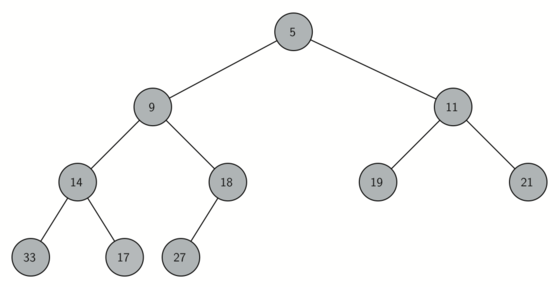
\includegraphics{figures/complete-binary-tree.png}

Another interesting property of a complete tree is that we can represent
it using a single list. We do not need to use nodes and references or
even lists of lists. Because the tree is complete, the left child of a
parent (at position \(p\)) is the node that is found in position \(2p\)
in the list. Similarly, the right child of the parent is at position
\(2p + 1\) in the list. To find the parent of any node in the tree, we
can simply use integer division (like normal mathematical division
except we discard the remainder). Given that a node is at position \(n\)
in the list, the parent is at position \(n/2\).

The diagram below shows a complete binary tree and also gives the list
representation of the tree. Note the \(2p\) and \(2p+1\) relationship
between parent and children. The list representation of the tree, along
with the full structure property, allows us to efficiently traverse a
complete binary tree using only a few simple mathematical operations. We
will see that this also leads to an efficient implementation of our
binary heap.

\hypertarget{the-heap-order-property}{%
\subsection{The Heap Order Property}\label{the-heap-order-property}}

The method that we will use to store items in a heap relies on
maintaining the heap order property. The \textbf{heap order property} is
as follows: In a heap, for every node \(x\) with parent \(p\), the key
in \(p\) is smaller than or equal to the key in \(x\). The diagram below
also illustrates a complete binary tree that has the heap order
property.

\begin{figure}
\centering
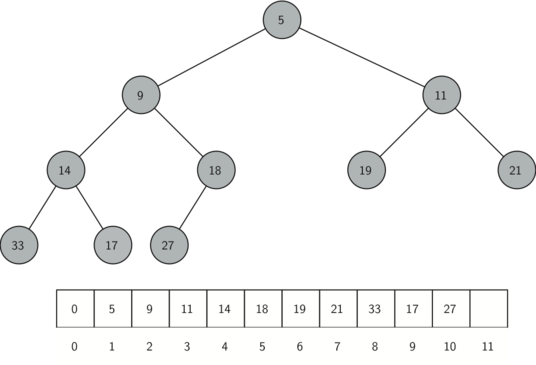
\includegraphics{figures/heap-order.png}
\caption{A complete binary tree, along with its list representation}
\end{figure}

\hypertarget{heap-operations}{%
\subsection{Heap Operations}\label{heap-operations}}

We will begin our implementation of a binary heap with the constructor.
Since the entire binary heap can be represented by a single list, all
the constructor will do is initialize the list and an attribute
\texttt{current\_size} to keep track of the current size of the heap.
The code below shows the Python code for the constructor. You will
notice that an empty binary heap has a single zero as the first element
of \texttt{items} and that this zero is not used, but is there so that
simple integer division can be used in later steps.

    \begin{tcolorbox}[breakable, size=fbox, boxrule=1pt, pad at break*=1mm,colback=cellbackground, colframe=cellborder]
\prompt{In}{incolor}{1}{\boxspacing}
\begin{Verbatim}[commandchars=\\\{\}]
\PY{k}{class} \PY{n+nc}{BinaryHeap}\PY{p}{(}\PY{n+nb}{object}\PY{p}{)}\PY{p}{:}
    \PY{k}{def} \PY{n+nf+fm}{\PYZus{}\PYZus{}init\PYZus{}\PYZus{}}\PY{p}{(}\PY{n+nb+bp}{self}\PY{p}{)}\PY{p}{:}
        \PY{n+nb+bp}{self}\PY{o}{.}\PY{n}{items} \PY{o}{=} \PY{p}{[}\PY{l+m+mi}{0}\PY{p}{]}

    \PY{k}{def} \PY{n+nf+fm}{\PYZus{}\PYZus{}len\PYZus{}\PYZus{}}\PY{p}{(}\PY{n+nb+bp}{self}\PY{p}{)}\PY{p}{:}
        \PY{k}{return} \PY{n+nb}{len}\PY{p}{(}\PY{n+nb+bp}{self}\PY{o}{.}\PY{n}{items}\PY{p}{)} \PY{o}{\PYZhy{}} \PY{l+m+mi}{1}
\end{Verbatim}
\end{tcolorbox}

    The next method we will implement is \texttt{insert}. The easiest, and
most efficient, way to add an item to a list is to simply append the
item to the end of the list. The good news about appending is that it
guarantees that we will maintain the complete tree property. The bad
news about appending is that we will very likely violate the heap
structure property. However, it is possible to write a method that will
allow us to regain the heap structure property by comparing the newly
added item with its parent. If the newly added item is less than its
parent, then we can swap the item with its parent. The diagram below
shows the series of swaps needed to percolate the newly added item up to
its proper position in the tree.

\begin{figure}
\centering
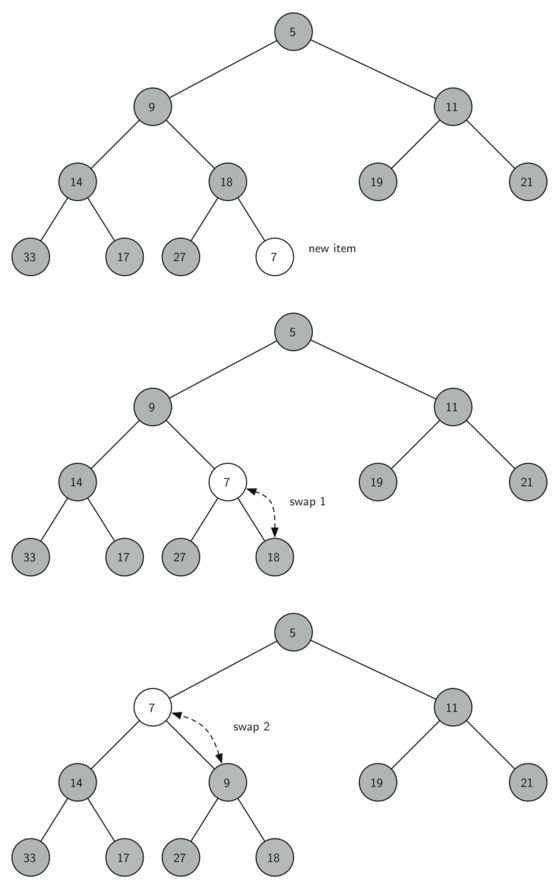
\includegraphics{figures/percolate-up.png}
\caption{Percolate the new node up to its proper position}
\end{figure}

Notice that when we percolate an item up, we are restoring the heap
property between the newly added item and the parent. We are also
preserving the heap property for any siblings. Of course, if the newly
added item is very small, we may still need to swap it up another level.
In fact, we may need to keep swapping until we get to the top of the
tree. The code below shows the \texttt{percolate\_up} method, which
percolates a new item as far up in the tree as it needs to go to
maintain the heap property. Here is where our wasted element in
\texttt{items} is important. Notice that we can compute the parent of
any node by using simple integer division. The parent of the current
node can be computed by dividing the index of the current node by 2.

    \begin{tcolorbox}[breakable, size=fbox, boxrule=1pt, pad at break*=1mm,colback=cellbackground, colframe=cellborder]
\prompt{In}{incolor}{2}{\boxspacing}
\begin{Verbatim}[commandchars=\\\{\}]
\PY{k}{def} \PY{n+nf}{percolate\PYZus{}up}\PY{p}{(}\PY{n+nb+bp}{self}\PY{p}{)}\PY{p}{:}
        \PY{n}{i} \PY{o}{=} \PY{n+nb}{len}\PY{p}{(}\PY{n+nb+bp}{self}\PY{p}{)}
        \PY{k}{while} \PY{n}{i} \PY{o}{/}\PY{o}{/} \PY{l+m+mi}{2} \PY{o}{\PYZgt{}} \PY{l+m+mi}{0}\PY{p}{:}
            \PY{k}{if} \PY{n+nb+bp}{self}\PY{o}{.}\PY{n}{items}\PY{p}{[}\PY{n}{i}\PY{p}{]} \PY{o}{\PYZlt{}} \PY{n+nb+bp}{self}\PY{o}{.}\PY{n}{items}\PY{p}{[}\PY{n}{i} \PY{o}{/}\PY{o}{/} \PY{l+m+mi}{2}\PY{p}{]}\PY{p}{:}
                \PY{n+nb+bp}{self}\PY{o}{.}\PY{n}{items}\PY{p}{[}\PY{n}{i} \PY{o}{/}\PY{o}{/} \PY{l+m+mi}{2}\PY{p}{]}\PY{p}{,} \PY{n+nb+bp}{self}\PY{o}{.}\PY{n}{items}\PY{p}{[}\PY{n}{i}\PY{p}{]} \PY{o}{=} \PYZbs{}
                    \PY{n+nb+bp}{self}\PY{o}{.}\PY{n}{items}\PY{p}{[}\PY{n}{i}\PY{p}{]}\PY{p}{,} \PY{n+nb+bp}{self}\PY{o}{.}\PY{n}{items}\PY{p}{[}\PY{n}{i} \PY{o}{/}\PY{o}{/} \PY{l+m+mi}{2}\PY{p}{]}
            \PY{n}{i} \PY{o}{=} \PY{n}{i} \PY{o}{/}\PY{o}{/} \PY{l+m+mi}{2}
\end{Verbatim}
\end{tcolorbox}

    We are now ready to write the \texttt{insert} method (see below). Most
of the work in the \texttt{insert} method is really done by
\texttt{percolate\_up}. Once a new item is appended to the tree,
\texttt{percolate\_up} takes over and positions the new item properly.

    \begin{tcolorbox}[breakable, size=fbox, boxrule=1pt, pad at break*=1mm,colback=cellbackground, colframe=cellborder]
\prompt{In}{incolor}{3}{\boxspacing}
\begin{Verbatim}[commandchars=\\\{\}]
\PY{k}{def} \PY{n+nf}{insert}\PY{p}{(}\PY{n+nb+bp}{self}\PY{p}{,} \PY{n}{k}\PY{p}{)}\PY{p}{:}
        \PY{n+nb+bp}{self}\PY{o}{.}\PY{n}{items}\PY{o}{.}\PY{n}{append}\PY{p}{(}\PY{n}{k}\PY{p}{)}
        \PY{n+nb+bp}{self}\PY{o}{.}\PY{n}{percolate\PYZus{}up}\PY{p}{(}\PY{p}{)}
\end{Verbatim}
\end{tcolorbox}

    With the \texttt{insert} method properly defined, we can now look at the
\texttt{delete\_min} method. Since the heap property requires that the
root of the tree be the smallest item in the tree, finding the minimum
item is easy. The hard part of \texttt{delete\_min} is restoring full
compliance with the heap structure and heap order properties after the
root has been removed. We can restore our heap in two steps. First, we
will restore the root item by taking the last item in the list and
moving it to the root position. Moving the last item maintains our heap
structure property. However, we have probably destroyed the heap order
property of our binary heap. Second, we will restore the heap order
property by pushing the new root node down the tree to its proper
position. The diagram shows the series of swaps needed to move the new
root node to its proper position in the heap.

\begin{figure}
\centering
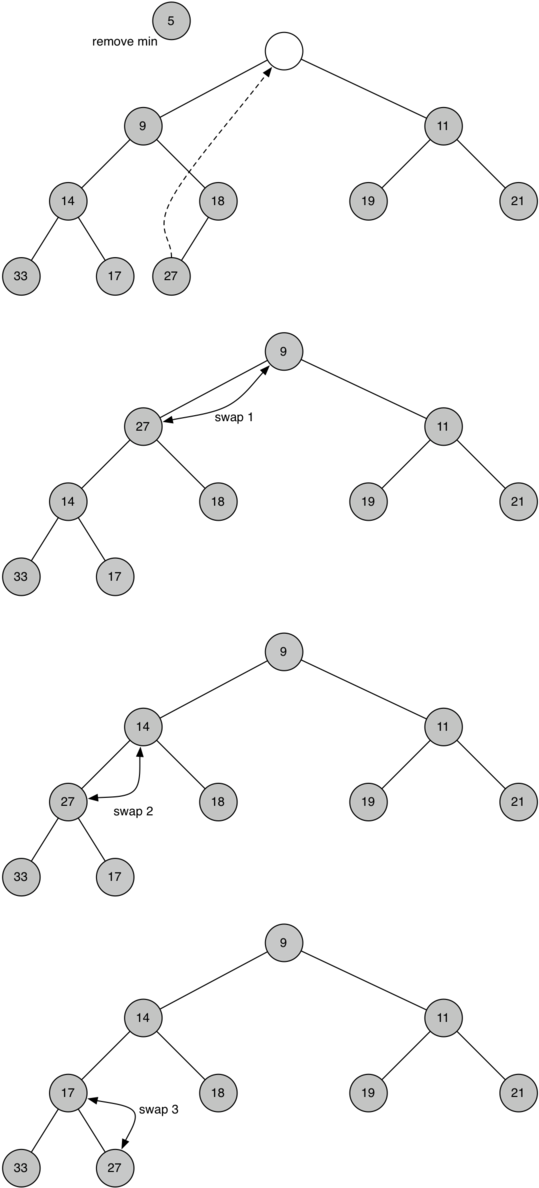
\includegraphics{figures/percolate-down.png}
\caption{Percolating the root node down the tree}
\end{figure}

In order to maintain the heap order property, all we need to do is swap
the root with its smallest child less than the root. After the initial
swap, we may repeat the swapping process with a node and its children
until the node is swapped into a position on the tree where it is
already less than both children. The code for percolating a node down
the tree is found in the \texttt{percolate\_down} and
\texttt{min\_child} methods below.

    \begin{tcolorbox}[breakable, size=fbox, boxrule=1pt, pad at break*=1mm,colback=cellbackground, colframe=cellborder]
\prompt{In}{incolor}{6}{\boxspacing}
\begin{Verbatim}[commandchars=\\\{\}]
\PY{k}{def} \PY{n+nf}{percolate\PYZus{}down}\PY{p}{(}\PY{n+nb+bp}{self}\PY{p}{,} \PY{n}{i}\PY{p}{)}\PY{p}{:}
        \PY{k}{while} \PY{n}{i} \PY{o}{*} \PY{l+m+mi}{2} \PY{o}{\PYZlt{}}\PY{o}{=} \PY{n+nb}{len}\PY{p}{(}\PY{n+nb+bp}{self}\PY{p}{)}\PY{p}{:}
            \PY{n}{mc} \PY{o}{=} \PY{n+nb+bp}{self}\PY{o}{.}\PY{n}{min\PYZus{}child}\PY{p}{(}\PY{n}{i}\PY{p}{)}
            \PY{k}{if} \PY{n+nb+bp}{self}\PY{o}{.}\PY{n}{items}\PY{p}{[}\PY{n}{i}\PY{p}{]} \PY{o}{\PYZgt{}} \PY{n+nb+bp}{self}\PY{o}{.}\PY{n}{items}\PY{p}{[}\PY{n}{mc}\PY{p}{]}\PY{p}{:}
                \PY{n+nb+bp}{self}\PY{o}{.}\PY{n}{items}\PY{p}{[}\PY{n}{i}\PY{p}{]}\PY{p}{,} \PY{n+nb+bp}{self}\PY{o}{.}\PY{n}{items}\PY{p}{[}\PY{n}{mc}\PY{p}{]} \PY{o}{=} \PY{n+nb+bp}{self}\PY{o}{.}\PY{n}{items}\PY{p}{[}\PY{n}{mc}\PY{p}{]}\PY{p}{,} \PY{n+nb+bp}{self}\PY{o}{.}\PY{n}{items}\PY{p}{[}\PY{n}{i}\PY{p}{]}
            \PY{n}{i} \PY{o}{=} \PY{n}{mc}

\PY{k}{def} \PY{n+nf}{min\PYZus{}child}\PY{p}{(}\PY{n+nb+bp}{self}\PY{p}{,} \PY{n}{i}\PY{p}{)}\PY{p}{:}
    \PY{k}{if} \PY{n}{i} \PY{o}{*} \PY{l+m+mi}{2} \PY{o}{+} \PY{l+m+mi}{1} \PY{o}{\PYZgt{}} \PY{n+nb}{len}\PY{p}{(}\PY{n+nb+bp}{self}\PY{p}{)}\PY{p}{:}
        \PY{k}{return} \PY{n}{i} \PY{o}{*} \PY{l+m+mi}{2}

    \PY{k}{if} \PY{n+nb+bp}{self}\PY{o}{.}\PY{n}{items}\PY{p}{[}\PY{n}{i} \PY{o}{*} \PY{l+m+mi}{2}\PY{p}{]} \PY{o}{\PYZlt{}} \PY{n+nb+bp}{self}\PY{o}{.}\PY{n}{items}\PY{p}{[}\PY{n}{i} \PY{o}{*} \PY{l+m+mi}{2} \PY{o}{+} \PY{l+m+mi}{1}\PY{p}{]}\PY{p}{:}
        \PY{k}{return} \PY{n}{i} \PY{o}{*} \PY{l+m+mi}{2}

    \PY{k}{return} \PY{n}{i} \PY{o}{*} \PY{l+m+mi}{2} \PY{o}{+} \PY{l+m+mi}{1}
\end{Verbatim}
\end{tcolorbox}

    The code for the \texttt{delete\_min} operation is below. Note that once
again the hard work is handled by a helper function, in this case
\texttt{percolate\_down}.

    \begin{tcolorbox}[breakable, size=fbox, boxrule=1pt, pad at break*=1mm,colback=cellbackground, colframe=cellborder]
\prompt{In}{incolor}{7}{\boxspacing}
\begin{Verbatim}[commandchars=\\\{\}]
    \PY{k}{def} \PY{n+nf}{delete\PYZus{}min}\PY{p}{(}\PY{n+nb+bp}{self}\PY{p}{)}\PY{p}{:}
        \PY{n}{return\PYZus{}value} \PY{o}{=} \PY{n+nb+bp}{self}\PY{o}{.}\PY{n}{items}\PY{p}{[}\PY{l+m+mi}{1}\PY{p}{]}
        \PY{n+nb+bp}{self}\PY{o}{.}\PY{n}{items}\PY{p}{[}\PY{l+m+mi}{1}\PY{p}{]} \PY{o}{=} \PY{n+nb+bp}{self}\PY{o}{.}\PY{n}{items}\PY{p}{[}\PY{n+nb}{len}\PY{p}{(}\PY{n+nb+bp}{self}\PY{p}{)}\PY{p}{]}
        \PY{n+nb+bp}{self}\PY{o}{.}\PY{n}{items}\PY{o}{.}\PY{n}{pop}\PY{p}{(}\PY{p}{)}
        \PY{n+nb+bp}{self}\PY{o}{.}\PY{n}{percolate\PYZus{}down}\PY{p}{(}\PY{l+m+mi}{1}\PY{p}{)}
        \PY{k}{return} \PY{n}{return\PYZus{}value}
\end{Verbatim}
\end{tcolorbox}

    To finish our discussion of binary heaps, we will look at a method to
build an entire heap from a list of keys. The first method you might
think of may be like the following. Given a list of keys, you could
easily build a heap by inserting each key one at a time. Since you are
starting with a list of one item, the list is sorted and you could use
binary search to find the right position to insert the next key at a
cost of approximately \(O(\log{n})\) operations. However, remember that
inserting an item in the middle of the list may require \(O(n)\)
operations to shift the rest of the list over to make room for the new
key. Therefore, to insert \(n\) keys into the heap would require a total
of \(O(n \log{n})\) operations. However, if we start with an entire list
then we can build the whole heap in \(O(n)\) operations. The code below
shows the code to build the entire heap.

    \begin{tcolorbox}[breakable, size=fbox, boxrule=1pt, pad at break*=1mm,colback=cellbackground, colframe=cellborder]
\prompt{In}{incolor}{8}{\boxspacing}
\begin{Verbatim}[commandchars=\\\{\}]
    \PY{k}{def} \PY{n+nf}{build\PYZus{}heap}\PY{p}{(}\PY{n+nb+bp}{self}\PY{p}{,} \PY{n}{alist}\PY{p}{)}\PY{p}{:}
        \PY{n}{i} \PY{o}{=} \PY{n+nb}{len}\PY{p}{(}\PY{n}{alist}\PY{p}{)} \PY{o}{/}\PY{o}{/} \PY{l+m+mi}{2}
        \PY{n+nb+bp}{self}\PY{o}{.}\PY{n}{items} \PY{o}{=} \PY{p}{[}\PY{l+m+mi}{0}\PY{p}{]} \PY{o}{+} \PY{n}{alist}
        \PY{k}{while} \PY{n}{i} \PY{o}{\PYZgt{}} \PY{l+m+mi}{0}\PY{p}{:}
            \PY{n+nb+bp}{self}\PY{o}{.}\PY{n}{percolate\PYZus{}down}\PY{p}{(}\PY{n}{i}\PY{p}{)}
            \PY{n}{i} \PY{o}{=} \PY{n}{i} \PY{o}{\PYZhy{}} \PY{l+m+mi}{1}
\end{Verbatim}
\end{tcolorbox}

    \begin{figure}
\centering
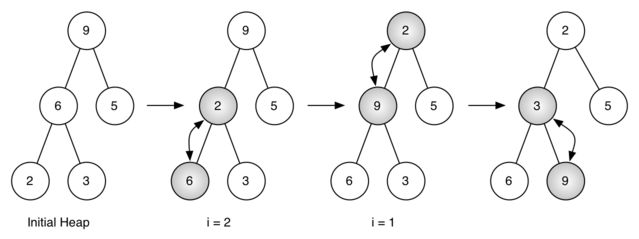
\includegraphics{figures/build-heap.png}
\caption{Building a heap from the list {[}9, 6, 5, 2, 3{]}}
\end{figure}

Above we see the swaps that the \texttt{build\_heap} method makes as it
moves the nodes in an initial tree of \texttt{{[}9,\ 6,\ 5,\ 2,\ 3{]}}
into their proper positions. Although we start out in the middle of the
tree and work our way back toward the root, the \texttt{percolate\_down}
method ensures that the largest child is always moved down the tree.
Because the heap is a complete binary tree, any nodes past the halfway
point will be leaves and therefore have no children. Notice that when
\texttt{i==1}, we are percolating down from the root of the tree, so
this may require multiple swaps. As you can see in the rightmost two
trees of above, first the 9 is moved out of the root position, but after
9 is moved down one level in the tree, \texttt{percolate\_down} ensures
that we check the next set of children farther down in the tree to
ensure that it is pushed as low as it can go. In this case it results in
a second swap with 3. Now that 9 has been moved to the lowest level of
the tree, no further swapping can be done. It is useful to compare the
list representation of this series of swaps as shown in above with the
tree representation.

\begin{verbatim}
i = 2  [0, 9, 5, 6, 2, 3]
i = 1  [0, 9, 2, 6, 5, 3]
i = 0  [0, 2, 3, 6, 5, 9]
\end{verbatim}

The assertion that we can build the heap in \(O(n)\) may seem a bit
mysterious at first, and a proof is beyond the scope of this book.
However, the key to understanding that you can build the heap in
\(O(n)\) is to remember that the \(\log{n}\) factor is derived from the
height of the tree. For most of the work in \texttt{build\_heap}, the
tree is shorter than \(\log{n}\).

    \begin{tcolorbox}[breakable, size=fbox, boxrule=1pt, pad at break*=1mm,colback=cellbackground, colframe=cellborder]
\prompt{In}{incolor}{ }{\boxspacing}
\begin{Verbatim}[commandchars=\\\{\}]

\end{Verbatim}
\end{tcolorbox}


    % Add a bibliography block to the postdoc
    
    
    
\end{document}
